\documentclass[11pt]{elegantbook}
\definecolor{structurecolor}{RGB}{40,58,129}
\linespread{1.6}
\setlength{\footskip}{20pt}
\setlength{\parindent}{0pt}
\newcommand{\argmax}{\operatornamewithlimits{argmax}}
\newcommand{\argmin}{\operatornamewithlimits{argmin}}
\elegantnewtheorem{proof}{Proof}{}{Proof}
\elegantnewtheorem{claim}{Claim}{prostyle}{Claim}
\DeclareMathOperator{\col}{col}
\title{\textbf{Analysis and Something Else}}
\author{Wenxiao Yang}
\institute{Haas School of Business, University of California Berkeley}
\date{2023}
\setcounter{tocdepth}{2}
\cover{cover.png}
\extrainfo{All models are wrong, but some are useful.}

% modify the color in the middle of titlepage
\definecolor{customcolor}{RGB}{9,119,119}
\colorlet{coverlinecolor}{customcolor}
\usepackage{cprotect}

\addbibresource[location=local]{reference.bib} % bib

\begin{document}

\maketitle
\frontmatter
\tableofcontents
\mainmatter


\chapter{Logic}
\section{Main Methods of Proof \small{ (@ Lec 01 of ECON 204)}}
\subsection{Proof by Induction}
\subsection{Proof by Deduction}
\subsection{Proof by Contradiction}
\subsection{Proof by Contraposition}
\begin{enumerate}[$\circ$]
    \item $\lnot P$ ("not $P$") means "$P$ is false".
    \item $P \wedge Q$ ("$P$ and $Q$") means “$P$ is true and $Q$ is true.”
    \item $P \vee Q$ ("$P$ or $Q$") means “$P$ is true or $Q$ is true (or possibly both).”
    \item $\lnot P \wedge Q$ means $(\lnot P)\wedge Q$; $\lnot P \vee Q$ means $(\lnot P)\vee Q$.
    \item $P \Rightarrow Q$ ("$P$ implies $Q$") means “whenever $P$ is satisfied, $Q$ is also satisfied.”
\end{enumerate}
\textbf{Statement:} Formally, $P \Rightarrow Q$ is equivalent to $\lnot P \vee Q$.

\begin{definition}[Contrapositive]
\normalfont
The \textit{contrapositive} of the statement $P \Rightarrow Q$ is the statement $\lnot Q \Rightarrow \lnot P$.
\end{definition}

\begin{theorem}[Prove Contrapositive Insead]
\normalfont
$P \Rightarrow Q$ is true if and only if $\lnot Q \Rightarrow \lnot P$ is true.
\end{theorem}



\chapter{Analysis Basis}
\section{Real Number $\mathbb{R}$ \small{(@ Lec 02 of ECON 204)}}
$\mathbb{R}$ is a field with the usual operations $+$, $\cdot$, additive identity $0$, and multiplicative identity $1$.
\subsection{Order Axiom}
\begin{proposition}[Order Axiom]
    \normalfont
    There is a complete ordering $\leq$, i.e. $\leq$ is reflexive, transitive, antisymmetric ($\alpha\leq\beta,\beta\leq\alpha \Rightarrow \alpha=\beta$) with the property that $\forall \alpha,\beta\in \mathbb{R}$ either $\alpha\leq\beta$ or $\beta\leq \alpha$.\\
    The order is compatible with $+$ and $\cdot$, i.e. $\forall \alpha,\beta,\gamma\in \mathbb{R}$
    \begin{enumerate}
        \item $\alpha\leq\beta \Rightarrow \alpha+\gamma\leq\beta+\gamma$.
        \item $\alpha\leq\beta,0\leq\gamma \Rightarrow \alpha\gamma\leq\beta\gamma$.
    \end{enumerate}
\end{proposition}

\subsection{Completeness Axiom}
\begin{proposition}[Completeness Axiom]\label{Completeness Axiom}
    \normalfont
    Suppose $L,H\subseteq \mathbb{R},L\neq\emptyset\neq H$ satisfy $\forall l\in L, h\in H$, $l\leq h$. Then, $$\exists\alpha\in \mathbb{R} \textnormal{ s.t. }\forall l\in L, h\in H,\ l\leq\alpha\leq h$$
\end{proposition}
\begin{center}\begin{figure}[htbp]
    \centering
    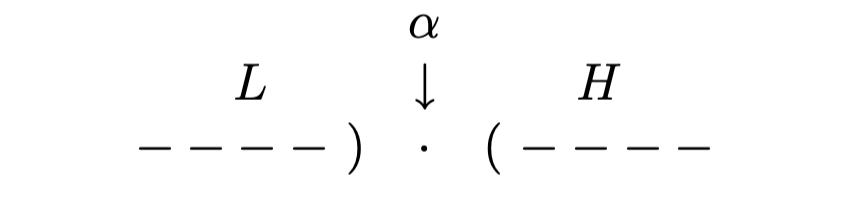
\includegraphics[scale=0.25]{CA.png}
    \caption{Completeness Axiom}
    \label{}
\end{figure}\end{center}

\begin{claim}
    \normalfont
    The Completeness Axiom differentiates $\mathbb{R}$ from $\mathbb{Q}$:\\
    $\mathbb{Q}$ satisfies all the axioms for $\mathbb{R}$ except the Completeness Axiom.
\end{claim}

\subsection{Supremum $\sup\mathbb{X}$, Infimum $\inf\mathbb{X}$ for $\mathbb{X}\subseteq \mathbb{R}$}
\begin{definition}[Supremum and Infimum]
    \normalfont
    \begin{enumerate}[(1).]
        \item Suppose $\mathbb{X}$ is bounded above. The \textbf{supremum} of $\mathbb{X}$, written $\sup\mathbb{X}$, is the least upper bound for $\mathbb{X}$, i.e. $\sup\mathbb{X}$ satisfies
        \begin{enumerate}
            \item $\sup\mathbb{X} \geq x,\forall x\in \mathbb{X}$ ($\sup\mathbb{X}$ is an upper bound).
            \item $\forall y<\sup\mathbb{X}$, $\exists x\in\mathbb{X}$ s.t. $x>y$ (there is no smaller upper bound).
        \end{enumerate}
        \item Suppose $\mathbb{X}$ is bounded below. The \textbf{infimum} of $\mathbb{X}$, written $\inf\mathbb{X}$, is the greatest lower bound for $\mathbb{X}$, i.e. $\inf\mathbb{X}$ satisfies
        \begin{enumerate}
            \item $\inf\mathbb{X} \leq x,\forall x\in \mathbb{X}$ ($\inf\mathbb{X}$ is a lower bound).
            \item $\forall y>\inf\mathbb{X}$, $\exists x\in\mathbb{X}$ s.t. $x<y$ (there is no greater lower bound).
        \end{enumerate}
        \item If $\mathbb{X}$ is not bounded above, write sup $\mathbb{X} = \infty$. If $\mathbb{X}$ is not bounded below, write inf $\mathbb{X} = -\infty$. By convention, $\sup \emptyset = -\infty$, $\inf \emptyset = +\infty$.
    \end{enumerate}
\end{definition}
\begin{proposition}
    If $\inf A=x^*\in A$ ($\sup A=x^*\in A$), then $x^*=\min A$ ($x^*=\max A$).
\end{proposition}

\subsection{The Supremum Property}
\begin{proposition}[The Supremum Property]\label{The Supremum Property}
    \normalfont
    Every nonempty set of real numbers that is bounded above has a supremum, which is a real number. Every nonempty set of real numbers that is bounded below has an infimum, which is a real number.
\end{proposition}

\begin{theorem}
    The Supremum Property (Prop \ref{The Supremum Property}) and the Completeness Axiom (Prop \ref{Completeness Axiom}) are equivalent.
\end{theorem}

\subsection{Archimedean Property}
\begin{theorem}[Archimedean Property]
    $\forall x\in \mathbb{R}, y\in \mathbb{R}^+$, $\exists n\in \mathbb{N}$ s.t. $ny>x$.
\end{theorem}

\section{Metric Spaces and Normed Spaces \small{(@ Lec 03 of ECON 204)}}
\subsection{Metric Space $(\mathbb{X}, d)$ and Metric $d : \mathbb{X} \times \mathbb{X} \rightarrow \mathbb{R}_+$}
\begin{definition}[Metric Space]
\normalfont
    A \textbf{metric space} is a pair $(\mathbb{X}, d)$, where $\mathbb{X}$ is a set and $d : \mathbb{X} \times \mathbb{X} \rightarrow \mathbb{R}_+$ a function satisfying
    \begin{enumerate}
        \item Non-negative: $d(x,y)\geq 0$, $d(x,y)=0\Leftrightarrow x=y, \forall x,y\in \mathbb{X}$.
        \item Symmetric: $d(x,y)=d(y,x), \forall x,y\in \mathbb{X}$.
        \item Triangle inequality: $d(x,z)\leq d(x,y)+d(y,z), \forall x,y,z\in \mathbb{X}$.
    \end{enumerate}
    A function $d : \mathbb{X} \times \mathbb{X} \rightarrow \mathbb{R}_+$ satisfying 1-3 is called a \textbf{metric} on $\mathbb{X}$.
\end{definition}
A metric gives a notion of distance between elements of $\mathbb{X}$.

\subsection{Norm $\|\cdot\|$ and Normed Vector Space $(V,\|\cdot\|)$}
\begin{definition}[Norm]
\normalfont
    Let $V$ be a vector space over $\mathbb{R}$. A \textbf{norm} on $V$ is a function $\|\cdot\| : V \rightarrow \mathbb{R}_+$ satisfying
    \begin{enumerate}
        \item Non-negative: $\|x\|\geq 0$, $\|x\|=0\Leftrightarrow x=0, \forall x\in V$.
        \item Triangle inequality: $\|x+y\|\leq \|x\|+\|y\|, \forall x,y\in V$.
        \item $\|\alpha x\|=|\alpha|\|x\|$, $\forall \alpha\in \mathbb{R},x\in V$.
    \end{enumerate}
\end{definition}
A norm gives a notion of length of a vector in $V$.

\begin{definition}[Normed Vector Space]
\normalfont
    A \textbf{normed vector space} is a vector space over $\mathbb{R}$ equipped with a norm, $(V,\|\cdot\|)$.
\end{definition}
\begin{example}[ Normed Vector Space]
\begin{enumerate}[-]
    \item $\mathbf{E}^n: n$-dimensional Euclidean space.
    $$
    V=\mathbb{R}^n,\|x\|_2=|x|=\sqrt{\sum_{i=1}^n\left(x_i\right)^2}
    $$
    \item $V=\mathbb{R}^n,\|x\|_1=\sum_{i=1}^n\left|x_i\right|$ (the "taxi cab" norm or $L^1$ norm)
    \item $V=\mathbb{R}^n,\|x\|_{\infty}=\max \left\{\left|x_1\right|, \ldots,\left|x_n\right|\right\}$ (the maximum norm, or sup norm, or $L^{\infty}$ norm)
    \item $C([0,1]),\|f\|_{\infty}=\sup \{|f(t)|: t \in[0,1]\}$
    \item $C([0,1]),\|f\|_2=\sqrt{\int_0^1(f(t))^2 d t}$
    \item $C([0,1]),\|f\|_1=\int_0^1|f(t)| d t$
\end{enumerate}
where $C([0,1])$ is the space of all continuous real-valued functions on $[0,1]$.
\end{example}

\subsection{Theorem: metric can be defined by norm}
In an abstract normed vector space, the norm can be used analogously to define a notion of distance.
\begin{theorem}
    Let $(V,\|\cdot\|)$ be a normed vector space. Let $d : \mathbb{X} \times \mathbb{X} \rightarrow \mathbb{R}_+$ be defined by $d(v, w) = \|v-w\|$. Then $(V, d)$ is a metric space.
\end{theorem}

\subsection{Cauchy-Schwarz Inequality}
\begin{theorem}[Cauchy-Schwarz Inequality]
    If $v, w \in \mathbb{R}^n$, then
    $$
    \begin{aligned}
    \left(\sum_{i=1}^n v_i w_i\right)^2 & \leq\left(\sum_{i=1}^n v_i^2\right)\left(\sum_{i=1}^n w_i^2\right) \\
    \|v \cdot w\|^2 & \leq\|v\|^2\|w\|^2 \\
    \|v \cdot w\| & \leq\|v\|\|w\|
    \end{aligned}
    $$
\end{theorem}

\subsection{Lipschitz-equivalent Norm}
\begin{definition}[Lipschitz-equivalent]
\normalfont
Two norms $\|\cdot\|$ and $\|\cdot\|^*$ on the same vector space $V$ are said to be \textbf{Lipschitz-equivalent} (or \textbf{equivalent}) if $\exists m,M>0$ s.t. $\forall x\in V$, $$m\|x\|\leq\|x\|^*\leq M\|x\|$$
Equivalently, $\exists m,M>0$ s.t. $\forall x\in V$, $x\neq 0$, $$m\leq\frac{\|x\|^*}{\|x\|}\leq M$$
\end{definition}
\begin{theorem}
    All norms on $\mathbb{R}^n$ are equivalent.
\end{theorem}
However, infinite-dimensional spaces support norms that are not equivalent. For example, on $C([0, 1])$, let $f_n$ be the function $$f_n(t)=\left\{\begin{matrix}
    1-nt,&\textnormal{if }t\in[0,\frac{1}{n}]\\
    0,&\textnormal{if }t\in(\frac{1}{n},1]
\end{matrix}\right.$$ Then $\frac{\|f_n\|_1}{\|f_n\|_\infty}=\frac{1}{2n}\rightarrow 0$, which means there is no lower bound $m>0$.

\subsection{Ball, Radius, Diameter, and Distance}
In a metric space $(X, d)$, define
$$
\begin{aligned}
B_{\varepsilon}(x) & =\{y \in X: d(y, x)<\varepsilon\} \\
& =\text { open ball with center } x \text { and radius } \varepsilon \\
B_{\varepsilon}[x] & =\{y \in X: d(y, x) \leq \varepsilon\} \\
& =\text { closed ball with center } x \text { and radius } \varepsilon
\end{aligned}
$$
We can use the metric $d$ to define a generalization of "radius". In a metric space $(X, d)$, define the \textit{diameter} of a subset $S \subseteq X$ by
$$
\operatorname{diam}(S)=\sup \left\{d\left(s, s^{\prime}\right): s, s^{\prime} \in S\right\}
$$
Similarly, we can define the \textit{distance from a point to a set}, and \textit{distance between sets}, as follows:
$$
\begin{aligned}
d(A, x) & =\inf _{a \in A} d(a, x) \\
d(A, B) & =\inf _{a \in A} d(B, a) \\
& =\inf \{d(a, b): a \in A, b \in B\}
\end{aligned}
$$

\section{Set Theory}
\subsection{Well Defined Set}
\begin{definition}
    A set $S$ is \textbf{well defined} if an object $a$ is either $a\in S$ or $a\notin S$.
\end{definition}

\subsection{Numerically Equivalent \small{(@ Lec 01 of ECON 204)}}
\begin{definition}
\normalfont
    Two sets $A, B$ are \textbf{numerically equivalent} (or have the same cardinality) if there is a bijection $f : A \rightarrow B$, that is, 1-1 ($a \neq a' \Rightarrow f(a) \neq f(a')$), and onto ($\forall b\in B, \exists a\in A$ s.t. $f(a)=b$).
\end{definition}

\subsection{Finite, Countable Set \small{(@ Lec 01 of ECON 204)}}
\begin{definition}[Finite Set]
\normalfont
    A set is either \textbf{finite} or \textbf{infinite}. A set is \textbf{finite} if it is \underline{numerically equivalent to} $\{1,...,n\}$ for some $n$. A set that is not finite is infinite.
\end{definition}

We give a more precise definition to classify infinite set:
\begin{definition}[Countable Set]
\normalfont
    An infinite set is \textbf{countable} if it is \underline{numerically equivalent to} $\mathbb{N}$. An infinite set that is not countable is called \textbf{uncountable}.
\end{definition}

\begin{theorem}[Countable $\mathbb{Q}$]
    The set of rational numbers $\mathbb{Q}$ is countable.
\end{theorem}


\subsection{Power Set \small{(@ Lec 02 of ECON 204)}}
\begin{definition}[Power Set: the set of all subsets]
    For any set $A$, we denote by $\mathcal{P}(A)$ the collection of all subsets of $A$. $\mathcal{P}(A)$ is the \textbf{power set} of $A$.
\end{definition}
We may also use the notation $2^A$ (in Berkeley ECON 204).

\subsection{Theorem (Cantor): The power set of $\mathbb{N}$ is uncountable \small{(@ Lec 02 of ECON 204)}}
\begin{theorem}[Cantor]
    $\mathcal{P}(\mathbb{N})$ (or denoted by $2^\mathbb{N}$), the set of all subsets of $\mathbb{N}$, is uncountable.
\end{theorem}

\subsection{Cardinalities of Sets \small{(@ Lec 02 of ECON 204)}}
\begin{definition}[Cardinality]
    If $A$ is a set, $|A|=$ cardinality of $A$ = $\#$ of elements
\end{definition}
$n \in \mathbb{N},|\{1, \ldots n\}|=n$; $|\emptyset|=0(\emptyset=\text { empty set })$.

\begin{proposition}[Facts about cardinality]
    \begin{enumerate}
        \item If $A$ is numerically equivalent to $\{1,...,n\}$ for some $n\in \mathbb{N}$, then $|A|=n$.
        \item $A$ and $B$ are numerically equivalent if and only if $|A|=|B|$.
        \item If $|A| = n$ (finite) and $A$ is a proper subset of $B$ (that is, $A\subset B$ and $A \neq B$) then $|A|<|B|$.
        \item If $A$ is countable and $B$ is uncountable, then $n<|A|<|B|, \forall n\in\mathbb{N}$.
        \item If $A\subseteq B$, then $|A|\leq|B|$. (if $B$ is countable and $A\subseteq B$, then $A$ is at most countable, that is, $A$ is either empty, finite, or countable.)
        \item If there is an \textit{injection} $\sigma:A \rightarrow B$, we can write $|A|\leq|B|$;
        \item If there is a \textit{surjection} $\sigma:A \rightarrow B$, we can write $|A|\geq|B|$;
        \item If there is a bijection $\sigma:A \rightarrow B$, we can write $|A|=|B|$.
    \end{enumerate}
\end{proposition}

\subsection{Pigeonhole Principle: $|A|>|B|$ $\Rightarrow$ no injective function $\sigma:A \rightarrow B$}
\begin{theorem}[Pigeonhole Principle]
    If $A$ and $B$ are sets and $|A|>|B|$, then there is no injective function $\sigma:A \rightarrow B$.
\end{theorem}



\subsection{$B^A$: Sets of Function}
If $A,B$ are sets, then $B^A=\{\sigma:A \rightarrow B| \sigma \textit{ a function}\}$.
\begin{example}
    $n\in \mathbb{Z}$, we define a function $f: B^{\{1,\dots,n\}} \rightarrow B^n(=B\times B\times B\times \dots \times B)$ by the equation
    $f(\sigma)=\{\sigma(1),...,\sigma(n)\}, \textit{ where }\sigma:\{1,\dots,n\} \rightarrow B$. The $f$ is a \textit{bijection}.
\end{example}
\begin{proof}
    \quad\\
    1. \textit{Injective}:
    \begin{equation}
        \begin{aligned}
            &f(\sigma_1)=f(\sigma_2)
            \Rightarrow \{\sigma_1(1),...,\sigma_1(n)\}=\{\sigma_2(1),...,\sigma_2(n)\}\\
            &\textit{Since }\sigma:\{1,\dots,n\} \rightarrow B,\textit{ it is sufficient to prove }\sigma_1=\sigma_2.
        \end{aligned}
        \nonumber
    \end{equation}
    2. \textit{Surjective}:
    \begin{equation}
        \begin{aligned}
            &\forall \{b_1,...,b_n\},\textit{ we have }\sigma^*(x)=b_x,x=1,...,n.\textit{ s.t. }f(\sigma^*)=\{b_1,...,b_n\}
        \end{aligned}
        \nonumber
    \end{equation}

\end{proof}
\begin{example}
    \begin{equation}
        \begin{aligned}
            & C(\mathbb{R},\mathbb{R})=\{\textit{continuous functions }\sigma:\mathbb{R} \rightarrow \mathbb{R} \}\subset \mathbb{R}^\mathbb{R}
        \end{aligned}
        \nonumber
    \end{equation}
\end{example}



\subsection{Bounded Set \small{(@ Lec 03 of ECON 204)}}
\begin{definition}[Bounded Set]
    \normalfont
    In a metric space $(X, d)$, a subset $S \subseteq X$ is \textbf{bounded} if $\exists x \in X, \beta \in \mathbb{R}$ such that $\forall s \in S$, $d(s, x) \leq \beta$.
\end{definition}



\subsection{Open, Closed Set \small{(@ Lec 04 of ECON 204)}}
\begin{definition}[Open Sets]
    Let $(X, d)$ be a metric space. A set $\mathbb{X} \subseteq \mathbb{R}^{n}$ is \textbf{open} if
    
    $\forall x \in \mathbb{X}$ we can draw a ball around $x$ that is contained in $\mathbb{X}$.

    i.e. $\forall x \in \mathbb{X}, \exists \varepsilon>0$ s.t. $B_\varepsilon(x)=\{y:d(y,x)<\varepsilon\} \subseteq \mathbb{X}$
\end{definition}

\begin{definition}[Closed Sets]
    $\mathbb{X}$ is \textbf{closed} if $\mathbb{X}^c$ is open.
\end{definition}
\begin{theorem}[Equivalent definition: Closed Sets]
    Equivalent: if $A$ in a metric space $(X, d)$ contains all limit points of all sequences in $A$, $A$ is closed.
    $$\{x_n\}\subset A, x_n \rightarrow x\in X \Rightarrow x\in A$$
\end{theorem}
\begin{example}[ (Closed and Open Sets on $\mathbb{E}_1$ i.e., $\mathbb{R}$ with the usual Euclidean metric)]
\end{example}
\begin{enumerate}[1)]
    \item $(1,2)=\{x \in \mathbb{R}: 1<x<2\}$ - open
    \item $\mathbb{R}$ is both open and closed
    \item $(-\infty, 1)=\{x \in \mathbb{R}: x<1\}$ - open
    \item $[1, \infty)$ is closed because its complement open
    \item $(1,2]$ is neither open nor closed
\end{enumerate}

\begin{example}[ (Closed and Open Sets on other metric space)]
    In the metric space $[0, 1]$, $[0, 1]$ is open. With $[0, 1]$ as the underlying metric space, $B_\varepsilon(0) = \{x \in [0, 1] : |x - 0| < \varepsilon\} = [0,\varepsilon)$.
\end{example}

\begin{theorem}
    [Empty Set and Full Set are both open and closed]
    In any metric space $(X, d)$ both $\emptyset$ and $X$ are open, and both $\emptyset$ and $X$ are closed.
\end{theorem}

\begin{theorem}[Union of open sets is open, Intersection of finite open sets is open]
    In any metric space $(X, d)$,
    \begin{enumerate}
        \item The union of an arbitrary (finite, countable, or uncountable) collection of open sets is open.
        \item The intersection of a finite collection of open sets is open.
    \end{enumerate}
\end{theorem}

\subsection{Interior, Exterior, Boundary, Closure \small{(@ Lec 04 of ECON 204)}}
Given a set $S\subseteq X$, the \textbf{point} of $X$ can be classified into three types relative to $S$:
\begin{enumerate}[$\bullet$]
    \item \textbf{Interior (points)}, denoted $int(S)$: $\vec{x}\in S$ for which there exists some $B(\vec{x},r)\subseteq S$, is the largest open set contained in $S$ (the union of all open sets contained in $S$).
    \item \textbf{Exterior (points)}, denoted $ext(S)$: $\vec{x}\notin S$ for which there exists some $B(\vec{x},r)$ containing \underline{no} points of $S$, is the largest open set contained in $X \backslash S$.
    \item \textbf{Boundary (points)} denoted $\partial (S)$ or $bd(S)$: all other points (for which any $B(\vec{x},r)$ will contain some points of $S$ and some points outside $S$).
    \item \textbf{Closure of $S$}, denoted $\bar{S}$ or $cl(S)=int(S)\cup bd(S)$,  is the smallest closed set containing $S$ (the intersection of all closed sets containing $S$).
    \item Moreover, boundary satisfies $\partial (S)=\overline{(X\backslash S)}\cap\bar{S}$.
\end{enumerate}

\begin{enumerate}[(1)]
    \item A set $S$ is \textbf{open} if $S=int(S)$ - i.e., if $S$ does \underline{not} contain any of its boundary points.
    \item A set $S$ is \textbf{closed} if $S=\bar{S}=int(S)\cup bd(S)$ - i.e., if $S$ contains \underline{all} of its boundary points.
\end{enumerate}

\subsection{Compact Set}
\begin{definition}[Compact Set]
    \normalfont
    $\mathbb{X} \subseteq \mathbb{R}^{n}$ is compact of it is closed and bounded.
\end{definition}

\begin{example}[ Compact Set]
    \normalfont
    $[1,2]=\{x \in \mathbb{R}: 1 \leqslant x \leqslant 2\}$; $\left\{x \in \mathbb{R}^{2}\right.: \left.x_{1}^{2}+x_{2}^{2} \leqslant 4\right\}$
\end{example}

\subsection{Sublevel Set}
\begin{definition}[Sublevel Set]
    \normalfont
    The sublevel set of a function $f: \mathbb{R}^n \rightarrow \mathbb{R}$ (for some level $c\in \mathbb{R}$) is the set $$\overline{L_c}=\{x\in \mathbb{R}^n:f(x)\leq c\}$$
\end{definition}



\subsection{Set Operations}
\begin{definition}
    \normalfont
    A \underline{binary operation} on a set $A$ is a function $*:A\times A \rightarrow A$.\\
    The \underline{operation is \textit{associative}} if $a*(b*c)=(a*b)*c, \forall a,b,c\in A$.\\
    The \underline{operation is \textit{commutative}} if $a*b=b*a, \forall a,b\in A$.
\end{definition}

\begin{example}

${+,\circ}$ are both \textit{associative} and \textit{commutative} operations on $\mathbb{Z},\mathbb{N},\mathbb{Q},\mathbb{R}$; $-$ is a neither \textit{associative} nor \textit{commutative} operation on $\mathbb{Z},\mathbb{Q},\mathbb{R}$, but not $\mathbb{N}$.
\end{example}

\begin{definition}
A subset $H\subset S$ is \underline{closed under $*$} if $a*b\in H$ for all $a,b\in H$.
\end{definition}

\begin{definition}
$*$ has \underline{identity element $e\in S$} if $a*e=e*a=a$ for all $s\in S$.
\end{definition}



\section{Sequences}
Sequences $\left\{x_{k}\right\}_{k=1}, \ldots$ or $\left\{x_{k}\right\}, x_{k} \in \mathbb{R}^{n}$

\begin{definition}[Subsequence]
\normalfont
    Suppose $\{x_n\}$ is a sequence and $n_1<n_2<\cdots$, then $\{x_{n_k}\}$ is called a \textbf{subsequence}.
\end{definition}

\subsection{Convergence of Sequences \small{(@ Lec 03 of ECON 204)}}
\begin{definition}[Convergence: note $x_{k} \rightarrow x, \lim _{k \rightarrow \infty} x_{k}=x$]
    Let $(X, d)$ be a metric space. A sequence $\{x_k\}$ converges to $x$ (written $x_{k} \rightarrow x$ or $\lim _{k \rightarrow \infty} x_{k}=x$) if $\forall \varepsilon>0, \exists N_{\varepsilon}$ s.t. $d(x_{k},x)<\varepsilon,\ \forall k \geqslant N_{\varepsilon}$
\end{definition}

\begin{definition}[Limit point]
    $x$ is a limit point of $\left\{x_{k}\right\}$ if $\exists \text { a subsequence of }\left\{x_{k}\right\} \text { that converges to } x$.
    \end{definition}
\begin{theorem}[Uniqueness of Limits]
    In a metric space $(X, d)$, if $x_{k} \rightarrow x$ and $x_{k} \rightarrow x'$, then $x=x'$.
\end{theorem}

\subsection{Cluster Point \small{(@ Lec 03 of ECON 204)}}
\begin{definition}[Cluster Point]
\normalfont
    An element $c$ is a \textbf{cluster point} of a sequence $\{x_n\}$ in a metric space $(X, d)$ if $\forall\varepsilon > 0, \{n : x_n \in B_\varepsilon(c)\}$ is an infinite set. Equivalently, $$\forall\varepsilon > 0, N\in \mathbb{N}, \exists n>N \textnormal{ s.t. } x_n \in B_\varepsilon(c)$$
\end{definition}
\begin{example}
    $x_n=\left\{\begin{matrix}
        1-\frac{1}{n},& \textnormal{ if $n$ even}\\
        \frac{1}{n},&\textnormal{ if $n$ odd}
    \end{matrix}\right.$ has cluster points $\{0,1\}$.
\end{example}

\begin{theorem}[Cluster Point $\Leftrightarrow$ exists subsequence converges to it]
    Let $(X, d)$ be a metric space, $c \in X$, and $\{x_n\}$ a sequence in $X$. Then $c$ is a cluster point of $\{x_n\}$ if and only if there is a subsequence $\{x_{n_k}\}$ such that $\lim_{k \rightarrow \infty} x_{n_k} = c$.
\end{theorem}

\subsection{Proposition: Sequences in $\mathbb{R}^n$, Bounded above and non-decreasing sequence $\Rightarrow$ Converge}
\begin{proposition}
    If $\left\{x_{k}\right\}$ is bounded above(below) and non-decreasing(non-increasing) it \textbf{converges}.
\end{proposition}

\subsection{Theorem: Increasing/Decreasing Sequences in $\mathbb{R}^n$, Limit is $\sup$/$\inf$ \small{(@ Lec 03 of ECON 204)}}

\begin{theorem}
    Let $\{x_n\}$ be an increasing (decreasing) sequence of real numbers. Then $\lim_{n \rightarrow \infty} x_n = \sup\{x_n : n \in \mathbb{N}\}$ ($\lim_{n \rightarrow \infty} x_n = \inf\{x_n : n \in \mathbb{N}\}$). In particular, the limit exists.
\end{theorem}

\subsection{Definition: $\lim\sup$ and $\lim\inf$ \small{(@ Lec 03 of ECON 204)}}
Consider a sequence $\{x_n\}$ of real numbers. Let $$\alpha_n=\sup\{x_k:k\geq n\}$$ and $$\beta_n=\inf\{x_k:k\geq n\}$$
Either $\alpha_n = +\infty$ for all $n$, or $\alpha_n \in \mathbb{R}$ and $\alpha_1 \geq \alpha_2 \geq \alpha_3 \geq...$. Either $\beta_n = -\infty$ for all n, or $\beta_n \in \mathbb{R}$ and $\beta_1 \leq \beta_2 \leq \beta_3 \leq ...$.
\begin{definition}[Lim Sups and Lim Infs]
    \normalfont
    $$
    \begin{aligned}
    & \limsup _{n \rightarrow \infty} x_n=\left\{\begin{array}{cl}
    +\infty & \text { if } \alpha_n=+\infty \text { for all } n \\
    \lim \alpha_n & \text { otherwise. }
    \end{array}\right. \\
    & \liminf _{n \rightarrow \infty} x_n=\left\{\begin{array}{cl}
    -\infty & \text { if } \beta_n=-\infty \text { for all } n \\
    \lim \beta_n & \text { otherwise. }
    \end{array}\right.
    \end{aligned}
    $$
\end{definition}

\subsection{Exists Limit $\Leftrightarrow$ $\lim=\lim\sup=\lim\inf$ \small{(@ Lec 03 of ECON 204)}}
\begin{theorem}
    Let $\left\{x_n\right\}$ be a sequence of real numbers. Then
    $$
    \begin{aligned}
    & \lim _{n \rightarrow \infty} x_n=\gamma \in \mathbf{R} \cup\{-\infty, \infty\} \\
    \Leftrightarrow & \lim \sup _{n \rightarrow \infty} x_n=\liminf _{n \rightarrow \infty} x_n=\gamma
    \end{aligned}
    $$
\end{theorem}

\subsection{Rising Sun Lemma: Sequence in $\mathbb{R}^n$ contains monotone subsequence \small{(@ Lec 03 of ECON 204)}}
\begin{theorem}[Rising Sun Lemma]
    Every sequence of real numbers contains an increasing subsequence or a decreasing subsequence or both.
\end{theorem}

\subsection{Bolzano-Weierstrass: Bounded Sequence in $\mathbb{R}^n$ contains a convergent subsequence \small{(@ Lec 03 of ECON 204)}}\label{B-W}
\begin{theorem}[Bolzano-Weierstrass]
    Every bounded sequence of real numbers contains a convergent subsequence.
\end{theorem}



\section{Complete Metric Spaces \small{(@ Lec 05 of ECON 204)}}
Roughly, a metric space is complete if “every sequence that ought to converge to a limit has a limit to converge to.”
\subsection{Cauchy Sequence}
\begin{definition}[Cauchy Sequence]
    A sequence $\{x_k\}$ in a metric space (X, d) is \textbf{Cauchy} if $\forall \varepsilon>0, \exists N(\varepsilon)$ s.t.
    $$d(x_{n},x_{m})<\varepsilon,\  \forall n, m > N(\varepsilon)$$
\end{definition}
\textbf{Note:} Cauchy property depends only on the sequence and the metric d, not on the ambient metric space.

\textbf{Note:} In $\mathbb{E}^1=(\mathbb{R},\|\cdot\|)$, $\left\{x_{k}\right\} \text { converges } \Longleftrightarrow\left\{x_{k}\right\} \text { is Cauchy}$.

A Cauchy sequence is trying really hard to converge, but there may not be anything for it to converge to. Any sequence that does converge must be Cauchy, however, by the argument above.

\subsection{Theorem: Convergent $\Rightarrow$ Cauchy}
\begin{theorem}[Convergent $\Rightarrow$ Cauchy]
    Every convergent sequence in a metric space is Cauchy.
\end{theorem}


\subsection{Complete Metric Space and Banach Space}
\begin{definition}[Complete Metric Spaces]
    \normalfont
    A metric space $(X, d)$ is \textbf{complete} if every Cauchy sequence $\{x_n\} \subseteq X$ converges to a limit $x \in X$.
\end{definition}
\begin{example}
    \begin{enumerate}
        \item Consider the earlier example of $X = (0, 1]$ with d the usual Euclidean metric. Since $x_n = \frac{1}{n}$ is Cauchy but does not converge in that metric space, $((0, 1], d)$ is not complete.
        \item $\mathbb{Q}$ is not complete in the Euclidean metric: $x_n=\frac{\left\lfloor 10^n \sqrt{2} \right\rfloor }{10^n} \rightarrow \sqrt{2}$.
    \end{enumerate}
\end{example}

\begin{definition}[Banach Space]
    \normalfont
    A \textbf{Banach space} is \textit{a normed space} that is complete in the metric generated by its norm.
\end{definition}

\begin{theorem}[$\mathbb{E}^1$ is complete]
    $\mathbb{R}$ is complete with the usual metric (so $\mathbb{E}^1$ is a Banach space).
\end{theorem}

\begin{theorem}[$\mathbb{E}^n$ is complete]
    $\mathbb{E}^n$ is complete for every $n \in \mathbb{N}$.
\end{theorem}

\begin{theorem}[$(C(X),\|\cdot\|_\infty)$ is Complete]
    Given $X \subseteq \mathbb{R}^n$, let $C(X)$ be the set of bounded continuous
    functions from $X$ to $R$ with $$\|f\|_\infty=\sup\{|f(x)|:x\in X\}$$
    Then $C(X)$ is a Banach space.
\end{theorem}

\subsection{Theorem: Subset of Complete Metric Space is Complete $\Leftrightarrow$ Subset is Closed}
\begin{theorem}[Subset of Complete Metric Space is Complete $\Leftrightarrow$ Subset is Closed]
    Suppose $(X, d)$ is a complete metric space and $Y \subseteq X$. Then $(Y, d) = (Y, d\mid_Y)$ is complete \underline{if and only if} $Y$ is a \textit{closed subset} of $X$. (where $d: \mathbb{X}\times \mathbb{X}\rightarrow \mathbb{R}_+$; $d\mid_Y: \mathbb{Y}\times \mathbb{Y}\rightarrow \mathbb{R}_+$)
\end{theorem}




\chapter{Functions}
\section{Definitions of Function}
\begin{definition}[Function]
    \normalfont
    \underline{\textit{Function}} is a rule $\sigma:A\rightarrow B$ that assigns an element $B$ to \textit{every} element of $A$. $\forall a\in A, \sigma(a)\in B$.
\end{definition}
\subsection{Image, Preimage, Fiber}
\begin{definition}
    \normalfont
\begin{enumerate}
    \item $A$ is the \underline{domain} of $\sigma$, $B$ is the \underline{range} of $\sigma$.
    \item We call $\sigma (a)= \textit{value of } \sigma\textit{ at } a$ as the \underline{image} of $a$.
    \item A set $C\subset B$, we call $\sigma^{-1}(C)=\{a\in A| \sigma(a)\in C\}$ as the \textit{\underline{preimage}} of $C$.
    \item An element $b\in B$, we call $\sigma^{-1}(b)=\{a\in A| \sigma(a)=b \}$ as the \textit{\underline{fiber}} of $b$.
\end{enumerate}
\end{definition}

\subsection{Composition of functions}
\begin{definition}[Function Composition]
\normalfont
The function composition $\circ$ is an operation that takes two functions $\sigma: A\rightarrow B$ and $\tau: B\rightarrow C$, , and produces a function $\tau\circ \sigma:A\rightarrow C$ that fulfills $\forall a\in A,\ (\tau\circ \sigma)(a)=\tau( \sigma(a))$.
\end{definition}

\subsection{Function Composition is Associative}
\begin{proposition}[Associativity of Functions]
    Suppose $\sigma:A \rightarrow B, \tau:B \rightarrow C, \rho:C \rightarrow D$ are functions and $\circ$ is the function composition, then $\rho\circ(\tau\circ\sigma)=(\rho\circ\tau)\circ\sigma$.
\end{proposition}


\subsection{Homeomorphism \small{(@ Lec 04 of ECON 204)}}
\begin{definition}[Homeomorphism]
    \normalfont
    Let $(X, d)$ and $(Y, \rho)$ be metric spaces. A function $f : X \rightarrow Y$ is called a \textbf{homeomorphism} if it is one-to-one, onto, continuous, and its inverse function is continuous.
\end{definition}

\section{Injection, Surjection, Bijection}
\subsection{Definitions: Injective, surjective, bijective}
A function $\sigma:A \rightarrow B$ is called,\\
1. \textit{Injective (1 to 1)}
\begin{equation}
    \begin{aligned}
        \forall a_1,a_2\in A, \sigma(a_1)=\sigma(a_2)\Rightarrow a_1=a_2
    \end{aligned}
    \nonumber
\end{equation}
2. \textit{Surjective (onto)}
\begin{equation}
    \begin{aligned}
        \forall b\in B,\exists a\in A, s.t. \sigma(a)=b
    \end{aligned}
    \nonumber
\end{equation}
3. \textit{Bijective} (if injective and surjective)

\subsection{Lemma 1.1.7: injective/surjective/bijective is preserved in composition}
\begin{lemma}[Lemma 1.1.7]
    Suppose $\sigma:A \rightarrow B, \tau: B \rightarrow C$ are functions,\\
    If $\sigma, \tau$ are injective, then $\tau\circ\sigma$ is \textit{injective}.\\
    If $\sigma, \tau$ are surjective, then $\tau\circ\sigma$ is \textit{surjective}.\\
    If $\sigma, \tau$ are bijective, then $\tau\circ\sigma$ is \textit{bijective}.
\end{lemma}

\subsection{Proposition 1.1.8: A function is bijection if there exist inverse}
\begin{proposition}[Proposition 1.1.8]
    A function $\sigma:A \rightarrow B$ is a bijection if $\exists$ a function $\tau:B \rightarrow A $ such that
    \begin{equation}
        \begin{aligned}
            &\sigma\circ\tau=id_B=\textit{identity on }B(id_B(x)=x, \forall x\in B)\\
            &\tau\circ\sigma=id_A
        \end{aligned}
        \nonumber
    \end{equation}
\end{proposition}
Such $\tau$ is unique, called inverse of $\sigma$, $\tau=\sigma^{-1}$.

\section{Function Continuity}

\subsection{Continuous Function in $\mathbb{R}$ with Euclidean norm}
\begin{definition}[Continunity at Point]
    \normalfont
    A real-valued function $f$ is \underline{\textbf{continuous} at $x$} if
    
    "For every $\left\{x_{k}\right\}$ converging to $x$ satisfies that $\lim _{k \rightarrow \infty} f\left(x_{k}\right)=f(x)$".

    Equivalent definition:

    $\forall \varepsilon>0, \exists \delta>0$ s.t.
    $\|y-x\|<\delta \Rightarrow |f(x)-f(y)|<\varepsilon$
\end{definition}
Continuity at $x_0$ requires:
\begin{enumerate}
    \item $f(x_0)$ is defined; and
    \item either
    \subitem - $x_0$ is an isolated point of $X$, i.e. $\exists \varepsilon > 0$ s.t. $B_\varepsilon(x) = \{x\}$; or
    \subitem - $\lim_{x \rightarrow x_0} f(x)$ exists and equals $f(x_0)$
\end{enumerate}

\begin{definition}[Continuous Function]
    \normalfont
    A real-valued function $f$ is \underline{continuous} if it is continuous at all points in its domain.
\end{definition}

\subsection{Continuous Function in Metric Spaces \small{(@ Lec 04 of ECON 204)}}
\begin{definition}[Continuity in Metric Spaces]
\normalfont
    Let $(X, d)$ and $(Y, \rho)$ be metric spaces. A function $f : X \rightarrow Y$ is \textbf{continuous} at a point $x_0 \in X$ if $\forall \varepsilon > 0, \exists \delta(x_0, \varepsilon) > 0$ s.t. $d(x, x_0) < \delta(x_0, \varepsilon) \Rightarrow  \rho(f(x), f(x_0)) < \varepsilon$.
\end{definition}

\subsection{Theorem: Continuous $\Leftrightarrow$ Preimage of open set is open \small{(@ Lec 04 of ECON 204)}}
\begin{theorem}[Continuous $\Leftrightarrow$ Preimage of open set is open]\label{Preimage of open set is open}
    Let $(X, d)$ and $(Y, \rho)$ be metric spaces, and $f : X \rightarrow Y$. Then $f$ is \textbf{continuous} if and only if
    $$f^{-1}(A)=\{x\in X: f(x)\in A\} \textnormal{ is open in $X$ $\forall A\subseteq Y$ s.t. $A$ is open in $Y$}$$
\end{theorem}

\subsection{Theorem: Continuity is preserved in composition \small{(@ Lec 04 of ECON 204)}}
\begin{theorem}[Continuity is preserved in composition]
    Let $(X, d_X)$, $(Y, d_Y)$ and $(Z, d_Z)$ be metric spaces. If $f : X \rightarrow Y$ and $g : Y \rightarrow Z$ are continuous, then $g \circ f : X \rightarrow Z$ is
    continuous.
\end{theorem}
\begin{proof}
    Proved by previous theorem \ref{Preimage of open set is open}.
\end{proof}

\subsection{Uniform Continuity \small{(@ Lec 04 of ECON 204)}}
\begin{definition}[Uniformly Continuous]
\normalfont
    Suppose $f : (X, d) \rightarrow (Y, \rho)$. $f$ is \textbf{uniformly continuous} if $$\forall \varepsilon>0, \exists \delta(\varepsilon)>0 \textnormal{ s.t. }\forall x_0\in X, d(x,x_0)<\delta(\varepsilon) \Rightarrow \rho(f(x), f(x_0))<\varepsilon$$
\end{definition}
\begin{claim}
    \textbf{Uniformly Continuous} implies (is stronger than) \textbf{Continuous}.\\
    ($f$ is continuous if $\forall x_0\in X, \varepsilon>0, \exists \delta(x_0,\varepsilon)>0 \textnormal{ s.t. } d(x,x_0)<\delta(x_0,\varepsilon) \Rightarrow \rho(f(x), f(x_0))<\varepsilon$)
\end{claim}
Given $\varepsilon>0$, "uniformly continuous" requires $\delta(\varepsilon)$ that works for all $x_0\in X$.



\subsection{Lipschitz Continuous \small{(@ Lec 04 of ECON 204)}}
\begin{definition}[Lipschitz (Continuous) in Normed Vector Space]
    Let $X, Y$ be normed vector spaces, $\mathbb{E} \subseteq X$.
    \begin{enumerate}[(1).]
        \item A function $f: X \rightarrow Y$ is \textbf{Lipschitz} on $\mathbb{E}$ satisfies
        $$\exists \gamma>0, 
        \|f(\mathbf{x})-f(\mathbf{y})\|_Y \leq \gamma\|\mathbf{x}-\mathbf{y}\|_X, \forall \mathbf{x}, \mathbf{y}\in \mathbb{E}
        $$
        or we call \textbf{$\gamma$-Lipschitz continuous};
        \item $f$ is \textbf{locally Lipschitz} on $\mathbb{E}$ if
        $$\forall x_0\in \mathbb{E}, \exists \varepsilon>0 \textnormal{ s.t. $f$ is Lipschitz on }B_\varepsilon(x_0)\cap \mathbb{E}$$
    \end{enumerate}
\end{definition}
\begin{claim}
    \begin{enumerate}[1).]
        \item If $f$ is $\gamma$-Lipschitz continuous, then it is also $(\gamma+1)$-Lipschitz continuous. The minimal such $\gamma$ is called a \underline{Lipschitz constant} of function $f$
        \item The definition can be extended to general metric spaces by replacing $\|\cdot\|_X$ and $\|\cdot\|_Y$ to general metrics.
    \end{enumerate}
\end{claim}

\begin{example}[ (Lipschitz)]
    \begin{enumerate}
        \item $f(x)=2 x$ is 2-Lipschitz continuous;
        \item What about $f(\mathbf{x})=\mathbf{A x}$, where $\mathbf{A}$ is a matrix? Spectral norm $\|\mathbf{A}\|_{2}$ (for Euclidean norm).
        \item What about $f(x)=x^{2}$ ?
        Not Lipschitz continuous, or the Lipschitz constant is $\infty$.
    \end{enumerate}
\end{example}
\begin{example}[ (Locally Lipschitz)]
    Every $C^1$ function is locally Lipschitz. (Recall that a function $f : \mathbb{R}^m \rightarrow \mathbb{R}^n$ is said to be $C^1$ if all its first partial derivatives exist and are continuous.)
\end{example}
\begin{claim}[Lipschitz continuity vs. continuity vs. uniform continuity]
    Lipschitz continuity is stronger than either continuity or uniform continuity:
    \begin{enumerate}[$\circ$]
        \item locally Lipschitz $\Rightarrow$ continuous
        \item Lipschitz $\Rightarrow$ uniformly continuous
    \end{enumerate}
\end{claim}

\subsection{Contraction (from the view of Lipschitz constant)}
\begin{enumerate}[a).]
    \item If the Lipschitz constant $\gamma \leq 1$, then $\mathrm{f}$ is called a \underline{non-expansive mapping}.
    \item If the Lipschitz constant  $\gamma<1$, then $f$ is called a \underline{contraction mapping}.
\end{enumerate}

\begin{example}
    \begin{enumerate}
        \item $f(x)=2 x$ is not a contraction mapping; $f(x)=0.5 x$ is.
        \item $f(x)=A x$ is a contraction mapping (with respect to Euclidean norm) iff $\|A\|_{2}<1$.
    \end{enumerate}
\end{example}

\section{Extreme Value, Intermediate Value of Functions}
\subsection{Intermediate Value Theorem \small{(@ Lec 02 of ECON 204)}}
\begin{theorem}[Intermediate Value Theorem]
    Suppose $f : [a, b] \rightarrow \mathbb{R}$ is continuous, and $f(a) < d < f(b)$. Then there exists $c \in (a, b)$ such that $f(c) = d$.
\end{theorem}

\subsection{Coercive Function}

\begin{definition}[Coercive]
    A real-valued function $f:\mathbb{X} \rightarrow \mathbb{R}$ is \underline{coercive} if for \textbf{every} $\left\{x_{k}\right\} \subset \mathbb{X}$ s.t. $\left\|x_{k}\right\| \rightarrow \infty, f\left(x_{k}\right) \rightarrow \infty$
\end{definition}

\begin{example}[ Check coercive]
\end{example}
1) $x \in \mathbb{R}^{2}, f(x)=x_{1}^{2}+x_{2}^{2}$ - coercive

2) $x \in \mathbb{R}, f(x)=1-e^{-|x|}$ - not coercive

3) $x \in \mathbb{R}^{2}, f(x)=x_{1}^{2}+x_{2}^{2}-2 x_{1} x_{2}$ - not coercive
(we need $f(x_k)\rightarrow	\infty$ for all $\left\|x_{k}\right\| \rightarrow \infty$)


\subsection{Extreme of Functions}
\begin{definition}[Extreme of Functions]
    Let $\mathbb{X} \subseteq \mathbb{R}^{n}, f: \mathbb{X} \rightarrow \mathbb{R}$
    $$\inf_{x \in \mathbb{X}} f(x)=\inf\{f(x): x \in \mathbb{X}\}$$
\end{definition}

If $\exists x^{*} \in \mathbb{X} \text { s.t. inf } f(x)=f\left(x^{*}\right)$. Then, $f$ achieves (attains) its minimum and $f\left(x^{*}\right)=\min _{x \in \mathbb{X}} f(x)$

$x^{*}$ is called a \textbf{minimizer} of $f$, written as $x^{*} \in \arg \min _{x \in \mathbb{X}} f(x)$. If $x^*$ is uniqne, we write $x^{*}=\arg \min _{x \in \mathbb{X}} f(x)
$

Similarly, supremum and maximum of $f$.

\subsection{Weierstrass' Theorem (Extreme value Theorem) \small{(@ Lec 05 of ECON 204)}}
\begin{theorem}
    [Weierstrass' Theorem (Extreme value Theorem)]
    \quad

    If $f$ is a \textbf{continuous} function on a \textbf{compact set}, $\mathbb{X} \subseteq \mathbb{R}^{n}$, then $f$ attains its min and max on $\mathbb{X}$ i.e.,
    $$
    \begin{aligned}
    \exists x_1 \in \mathbb{X} \text { s.t. } f\left(x_{1}\right) &=\inf _{x \in \mathbb{X}} f(x) \\
    \exists x_{2} \in \mathbb{X} \text { s.t. } f\left(x_{2}\right) &=\sup _{x \in \mathbb{X}} f(x)
    \end{aligned}
    $$
\end{theorem}
\begin{proof}
    (for existence of $\min$; $\max$ is similar)

    Let $\{\sigma_k\}\subseteq \mathbb{X}$ be s.t.
    $\inf_{x\in\mathbb{X}} f(x) \leq f\left(\sigma_{k}\right) \leq \inf _{x \in \mathbb{X}} f(x)+\frac{1}{k}$

    Then $\lim _{k \rightarrow \infty} f\left(\sigma_{k}\right)=\inf_{x\in\mathbb{X}} f(x)$

    $\mathbb{X}$ is bounded $\Rightarrow\left\{\sigma_{k}\right\}$ has it least one limit point $x_1$,

    $\mathbb{X}$ is closed $\Rightarrow x_{1} \in \mathbb{X}$

    $f$ is continuous $\Rightarrow f\left(x_{1}\right)=\lim _{k \rightarrow \infty} f\left(\sigma_{k}\right)=\inf _{x \in \mathbb{X}} f(x)$
\end{proof}

\begin{corollary}[Corollary to WT]
    Let $f$ be continuous on closed set $\mathbb{X}$ (not necessarily bounded). If $f$ is coercive on $\mathbb{X}$ it attains its $\min$ on $\mathbb{X}$.
\end{corollary}
\begin{proof}
    Consider $\left\{\sigma_{k}\right\}$ as in proof of $WT$.

    Since $f$ is closed, $f(x)<\infty,\ \forall x\in\mathbb{X}$. And $f$ is coercive on $\mathbb{X}$, which means $f(x)\rightarrow \infty$ if $\|x\| \rightarrow\infty$. Hence, $\left\{\sigma_{k}\right\}\in\mathbb{X}$ is bounded. Rest of proof same as proof of $\mathrm{WT}$.
\end{proof}

\begin{example}
    $f(x)=f\left(x_{1}, x_{2}, x_{3}\right)=x_{1}^{4}+2 x_{2}^{2}+e^{-x_{3}}+e^{2 x_{3}}$
\end{example}

\begin{enumerate}[1)]
    \item \textit{Does $f$ achieve its $\min$ and $\max$ on $\mathbb{X}_{1}=\left\{x \in \mathbb{R}^{3}: x_{1}^{2}+2 x_{2}^{2}+3 x_{3}^{2} \leqslant 6\right\}$?}
    
    - $\mathbb{X}_{1}$ is compact and $f$ is continuous. Both $\min$ and $\max$ are achieved (WT).
    \item Does $f$ achieve its min and max over $\mathbb{R}^{3}$?
    
    - $f \rightarrow \infty$ whenever $\|x\| \rightarrow \infty \Rightarrow f$ is coercive.

    - $\mathbb{R}^{3}$ is closed.

    $\Rightarrow f$ achieves its min. on $\mathbb{R}^{3}$ by corollary to WT.

    - $\max$ does not exist since $f \rightarrow \infty$ as $\|x\| \rightarrow \infty$.

    \item Does $f$ achieve its min and max over $\mathbb{X}_{2}=\{x \in \mathbb{R}^{3}: x_{1}+x_{2}+x_{3}=3\}$?
    
    - $\mathbb{X}_{2}$ is closed, but not bounded.

    - Since $f$ is coercive, $\min$ achieved.

    - $\max$ does not exist since setting $x_{1}=0$ $x_{2}=3-x_{3}$ and letting $x_{3} \rightarrow \infty$ makes $f \rightarrow \infty$
\end{enumerate}


\section{Monotonic Function \small{(@ Lec 05 of ECON 204)}}
\begin{definition}
    \normalfont
    A function $f : \mathbb{R} \rightarrow  \mathbb{R}$ is \textbf{monotonically increasing} if $y>x \Rightarrow f(y)\geq f(x)$.
\end{definition}

\subsection{Theorem: Monotonically Increasing $\Rightarrow$ One-sided Limits exist}
\begin{theorem}
    Let $a, b \in \mathbb{R}$ with $a < b$, and let $f : (a, b) \rightarrow \mathbb{R}$ be monotonically increasing. Then the one-sided limits: $f(t^+)=\lim_{u \rightarrow t^+}f(u)$ and $f(t^-)=\lim_{u \rightarrow t^-}f(u)$ exist and are real numbers for all $t \in (a, b)$.
\end{theorem}
\begin{center}\begin{figure}[htbp]
    \centering
    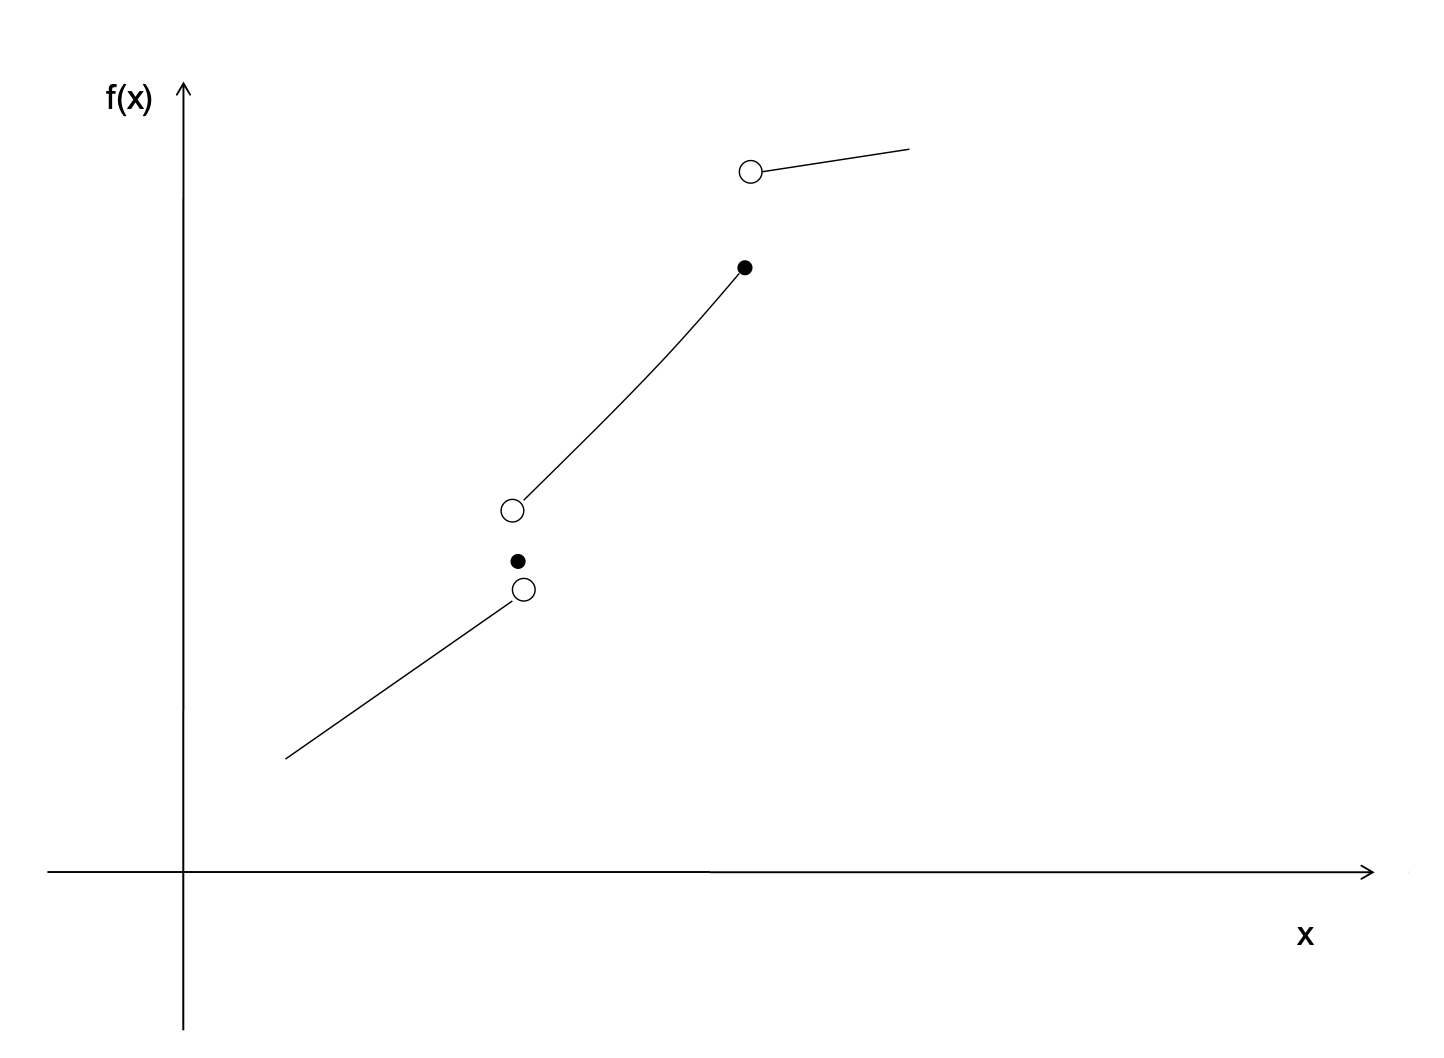
\includegraphics[scale=0.2]{SJD.png}
    \caption{A monotonic function has only simple jump discontinuities.}
    \label{}
\end{figure}\end{center}

\subsection{Theorem: Monotonically Increasing $\Rightarrow$ Set of Points are discontinuous is finite (possibly empty) or countable}
\begin{theorem}
    Let $a, b \in \mathbb{R}$ with $a < b$, and let $f : (a, b) \rightarrow \mathbb{R}$ be monotonically increasing. Then $D=\{t\in(a,b): f \textnormal{ is discontinuous at }t\}$ is finite (possibly empty) or countable.
\end{theorem}

\section{Contraction Mapping Theorem}
\subsection{Contractions}
\begin{definition}
    \normalfont
    Let $(X, d)$ be a \underline{nonempty complete} metric space. An operator is a function $T : X \rightarrow X$. An operator $T$ is a \textbf{contraction of modulus $\beta$} if $\beta < 1$ and $$d(T(x), T(y)) \leq \beta d(x, y), \forall x,y\in X$$
\end{definition}
A contraction shrinks distances by a \textit{uniform} factor $\beta < 1$.

\subsection{Theorem: Contraction $\Rightarrow$ Uniformly Continuous}
\begin{theorem}[Contraction $\Rightarrow$ Uniformly Continuous]
    Every contraction is uniformly continuous.
\end{theorem}
\begin{proof}
    Let $\delta=\frac{\varepsilon}{\beta}$.
\end{proof}


\section{Fixed Point Theorem}
\subsection{Fixed Point}
\begin{definition}[Fixed Point]
    \normalfont
    A \textbf{fixed point} of an operator $T$ is element $x^*\in X$ such that $T(x^*)=x^*$.
\end{definition}

\subsection{Contraction Mapping Theorem}
\begin{theorem}[Contraction Mapping Theorem]
    Let $(X, d)$ be a nonempty complete metric space and $T : X \rightarrow X$ a contraction with modulus $\beta < 1$. Then
    \begin{enumerate}
        \item $T$ has a unique fixed point $x^*$.
        \item For every $x_0 \in X$, the sequence defined by
        \begin{equation}
            \begin{aligned}
                x_1&=T(x_0)\\
                x_2&=T(x_1)=T(T(x_0))=T^2(x_0)\\
                &\vdots\\
                x_{n+1}&=T(x_n)=T^{n+1}(x_0)
            \end{aligned}
            \nonumber
        \end{equation}
    \end{enumerate}
\end{theorem}
\begin{proof}
\end{proof}





\chapter{Big $\mathcal{O}$ and Small $o$ Notation}
\section{Definition}
\begin{center}
    \fcolorbox{black}{gray!10}{\parbox{.9\linewidth}{\textbf{\underline{Complexity}:}
    \begin{definition}
        A sequence $f(n)$ is $O(1)$ if $\lim_{n \rightarrow \infty}f(n)<\infty$.
    \end{definition}
    
    \begin{definition}
        A sequence $f(n)$ is $O(g(n))$ if $\frac{f(n)}{g(n)}$ is $O(1)$.
    \end{definition}
    
    \begin{definition}
        A sequence $f(n)$ is $o(1)$ if $\lim_{n \rightarrow \infty}\sup f(n)=0$.
    \end{definition}
    
    \begin{definition}
        A sequence $f(n)$ is $o(g(n))$ if $\lim_{n \rightarrow \infty}\sup \frac{f(n)}{g(n)}=0$.
    \end{definition}
    
    \begin{definition}
        A sequence $f(n)$ is \underline{asymptotic} to $g(n)$ if $\lim_{n \rightarrow \infty} \frac{f(n)}{g(n)}=1$. (This is denoted by $f(n)\sim g(n)$ as $a \rightarrow \infty$)
    \end{definition}
    }}
\end{center}
For two scalar functions $f(x)\in \mathbb{R}, g(x)\in \mathbb{R}_+$, where $x\in \mathbb{R}$, we write:
\begin{enumerate}
    \item $f(x)=\mathcal{O}(g(x))$ if $\lim \sup_{x \rightarrow	\infty}\frac{|f(x)|}{g(x)}<\infty$; we say $f$ is dominated by $g$ asymptotically.
    \item $f(x)=\Omega(g(x))$ if $\lim \inf_{x \rightarrow \infty}\frac{|f(x)|}{g(x)}>0$.
    \item $f(x)=\Theta (g(x))$ if $f(x)=\mathcal{O}(g(x))$ and $f(x)=\Omega(g(x))$ both hold.
    \item $f(x)=o(g(x))$ if $\lim \inf_{x \rightarrow \infty}\frac{f(x)}{g(x)}=0$.
\end{enumerate}

\begin{example}
\begin{equation}
    \begin{aligned}
        n^3+n+2=\Omega(1),n^3+n+2=\Omega(n^2)\\
        n^3+n+2=\Theta(n^3)\\
        n^3+n+2=o(n^4)
    \end{aligned}
    \nonumber
\end{equation}
\end{example}

\subsection{Extension}
$f(x)=\mathcal{O}(g(x))$ as $x \rightarrow a$ if $\lim \sup_{x \rightarrow a}\frac{|f(x)|}{g(x)}<\infty$.

\begin{example}
$\varepsilon^2+\varepsilon^3=\mathcal{O}(\varepsilon^2)$ as $\varepsilon \rightarrow 0$
\end{example}


\chapter{Fixed point theorem}
1. Fixed point theorem: If $f$ is a contraction mapping that maps $\mathbb{R}^{n}$ to itself, then the following two results hold:

1) There exists a unique fixed point $\mathrm{x}^{*}$ satisfying
$$
\mathbf{x}^{*}=f\left(\mathbf{x}^{*}\right)
$$
2) In addition, the iterated function sequence
$$
\mathbf{x}, f(\mathbf{x}), f(f(\mathbf{x})), \cdots \text {, }
$$
converges to this unique fixed point $\mathbf{x}^{*}$ (independent of the initial point $x$ ).

2. Remark: This is a special case of "Banach fixed point theorem" (which applies to any complete metric space).









\end{document}